\documentclass{article}
\usepackage[utf8]{inputenc}
\usepackage{graphicx}
\usepackage[margin=1.0in]{geometry}
\usepackage{float}
\usepackage{wrapfig}
\usepackage{textcomp}
\usepackage{mathtools, nccmath}
\usepackage{amssymb}
\usepackage{amsmath}
\usepackage{mathrsfs}
\usepackage{dsfont}
\usepackage{lmodern}
\usepackage{textcomp}
\usepackage{hyperref}
\usepackage{physics}
\usepackage{listings}
\setlength{\parindent}{0pt}
\usepackage{setspace}
\usepackage[sorting=none]{biblatex}
\usepackage{caption}
\usepackage{subcaption}
\usepackage[eng]{nbi}
%\addbibresource{lit.bib}
\onehalfspacing

\supervisor{Klaus Mølmer}
\project{Project outside course scope}
\author{Emil H. Henningsen}
\title{Investigation of Collective Atomic Excitation States}
\subtitle{}
\institute{Niels Bohr Institute}
\department{Hy-Q - Center for Hybrid Quantum Networks}
\email{tzs820@alumni.ku.dk}
\handindate{$14^{th}$ of June, 2024}
\defencedate{$21^{st}$ of June, 2024}

\begin{document}

\maketitle

\section*{Abstract}

TODO. 

\section*{Acknowledgements}

\newpage
\tableofcontents

\section{Introduction}

The collective excitation states of an atomic array is a well-known phenomenon in the physics of light-matter interaction (REF). In the field of quantum information processing, long-lived quantum states are desired for implementing both quantum communication protocols and quantum computing. Certain excited states of atomic arrays display greatly amplified (superradiant) or suppresed (subradiant) decay rates, when compared to a single atom in vacuum. Such states arise in the interplay of atoms arranged closely together and the surrounding electromagnetic field. In the following, exciting new geometries and variations are investigated within the scope of finding highly subradiant states. The model used for these calculations is a second quantized approach, in which the atoms are assumed dipoles, and the suppresed radiance is manifested as destructive interference between these (???). Furthermore, theoretical considerations are presented to elaborate on expectations and results of these calculations. This project is restricted to radiation in free-space. 

Hvad er mine quantities of interest?

\section{Theory}\label{sec:theory}

The model is developed from a classical perspective, but will in the end be used to describe the quantized field and therefore be a fully quantum model (REF Gruner og Welsch). The model is used to describe the interaction between atoms and the empty-space electromagnetic field. The model is capable of describing both homogenous and inhomogenous Kramers-Kronig dielectrics (REF Gruner og Welsch), which makes it desirable for in-depth studies of collectively excited atomic arrays in various settings and environments. Due to the quantities of interest in this project, the framework is restricted to free space in the following. 

List of assumptions and approximations (REF Asenjo):
\begin{itemize}\label{list:assumptions}
    \item All photons are mediated in vacuum, i.e. $\varepsilon(\bar{r},\omega) = \varepsilon_0$,
    \item Targeting a single transition in the atoms (two-level system), the dipole-interaction between atoms and the field happens at a narrow band-width, i.e. $\omega \rightarrow \omega_0$,
    \item The atoms are tightly trapped, such that their positions can be treated as stationary points. 
    \item Interatomic distances are smaller than the wavelength of emitted photons, $d < \lambda_0$. With this, the retardation of the field between the atoms can be neglected, 
    \item There are no strongly-coupled modes between the field and the atoms (which would e.g. be the case, if the atoms were placed in an optical cavity). Together with the abovementioned assumption, the emission is in the Markovian regime, which means "the system will have no memory of its past" (REF Deutsch) once the photon has escaped. 
\end{itemize}
The latter two points allow for the promotion of field and dipole moment to quantum operators, after which the field described by Green's tensor and radiation-scattering dipoles can be coherently described by atomic coherence operators. In particular, the Green's tensor under these assumptions become (REF Asenjo, Equation 6):

\begin{equation}\label{eq:Greens}
    \underline{G}_0 (\bar{r}_{ij}, \omega_0) = \frac{e^{ik_0r}}{4\pi k_0^2 r^3} \cdot \left[ (k_0^2r^2 + ik_0r - 1) \mathds{1}_3 + (-k_0^2 r^2 -3ik_0r + 3) \frac{\ket{\bar{r}_{ij}}\bra{\bar{r}_{ij}}}{r^2} \right].
\end{equation}
Where $r$ is the norm of the displacement between atoms i and j: $\bar{r}_{ij}$, $k_0=\frac{\omega_0}{c}$ is the norm of the wave vector, $\mathds{1}_3$ is the three-dimensional identity matrix and $\ket{\bar{r}_{ij}}\bra{\bar{r}_{ij}}$ is the outer product of the displacement vector. 

The effective Hamiltonian (REF Asenjo), which is subject to diagonalization:
\begin{equation}\label{eq:Heff}
    \begin{split}
        \hat{H}_{eff} &= - \mu_0 \cdot \omega_0^2 \cdot \sum_{i,j = 1}^N \bar{\mathscr{D}}^\dagger \underline{G}_0(\bar{r_i}, \bar{r_j}, \omega_0) \bar{\mathscr{D}} \sigma_+^i \sigma_-^j, \\
        &=- \mu_0 \cdot \omega_0^2 \cdot \|\bar{\mathscr{D}}\|^2 \cdot \sum_{i,j = 1}^N \hat{n}^T \underline{G}_0(\bar{r_i}, \bar{r_j}, \omega_0) \hat{n} \sigma_+^i \sigma_-^j. \\
    \end{split}
\end{equation}
Where $\mu_0$ is the vacuum permeability, $\omega_0$ is the atomic transition frequency, $\bar{\mathscr{D}}$ is the dipole vector at atom j (however, for most applications, equal directioned dipoles are chosen) and $\sigma_\pm^i$ is the i'th atom's coherence operators acting on the i'th subspace of full Hilbert space. In the last line, the dipole amplitude is separated from the direction, which proves useful when converting to a dimensionless model in Section \ref{sec:dimless}. This matrix fully describes the atom-atom interaction in a quantum jump formalism (REF Asenjo). However, this is not the entire description of the system. At some point, a photon mode is excited, and the excitation is lost to the system. This reflects in the fact that the above matrix is non-Hermitian, i.e. $\hat{H}_{eff} \neq \hat{H}_{eff}^\dagger$. Hermitian matrices conserve norm, meaning no probability amplitude leaves the system. In this description, probability amplitude "leaks" away, as the probability of exciting an photon mode increases. If the system is initialized with an excitation, then at $t=0$, the eigenvectors are the actual eigenstates of the system, even though the non-Hermiticity dictates the non-existence of a single orthonormal basis for the singular value decomposition. It is therefore still valid to consider the eigenvectors, and of particular interest in this project the eigenvalues, of the effective Hamiltonian. The eigenvalues of this matrix are complex numbers, where the real part corresponds to a finite energyshift due to the atoms being close together, and the imaginary part corresponds to damping in time of the state, i.e. decay rates (REF Asenjo, Equation 7): $\lambda_\xi = J_\xi - \frac{i}{2} \Gamma_\xi$. The steps taken towards diagonalizing the matrix is described in Section \ref{sec:block}. 

Another issue must also be adressed before working with the abovementioned framework. It is evident in Equation \ref{eq:Greens} that the diagonal values diverge, when the distance goes to zero. The diagonal values describe the interaction of the atoms with themselves, i.e. if they were to be alone, $N = 1$, there should be no energy shift, and the decay rate must be the well-known spontaneous vacuum emission rate:

\begin{equation}\label{eq:vac_emission_rate}
    \Gamma_0 = \frac{\omega_0^3}{3\pi \hbar \varepsilon_0 c^3} \cdot \|\bar{\mathscr{D}}\|^2
\end{equation}

Therefore, the diagonal values of $\hat{H}_{eff}$ are but a constant offset of the identity, which gives the full matrix:

\begin{equation}
    \hat{H} = \sum_{i=0}^N (\hbar \omega_0 - \frac{i}{2}\Gamma_0) \hat{\sigma}_{ee}^{i} -\mu_0 \omega_0^2 \|\bar{\mathscr{D}}\|^2 \sum_{i,j = 1, i \neq j}^N \hat{n}^T \underline{G}_0(\bar{r}_{ij}, \omega_0) \hat{n} \sigma_+^i \sigma_-^j.
\end{equation}
NOTE: Ved ikke lige med denne del.... Skal i hvert fald inkludere noget omkring diagonalen indsættes ved håndkraft.

In general, becuase the atomic transitions are well-defined two-level systems, this formalism can be considered as spin-wave excitations in arrays of spin-½ particles. This does not give any more clarity on the behaviour of the system for single excitation states, as this is equivalently described by interference between the dipoles. It is another case, when considering multiple excitation states, as the fermionic nature of spin-½ particles gives rise to interesting dynamics (REF Asenjo, Section IIIC). In this project, the quantities of interest limits the use of the formalism to the single-excitation manifold, but multiple excitations is one of the directions outlined as further research in Section \ref{sec:further}. 

Kæde: Foton kan ikke undslippe ortogonalt til kæden. Hvorfor? -> "Spin-bølge" tilstand i gitteret. -> faststoffysik-sprog. Subradiante tilstande for bølgevektorer indenfor første Brillouin-zone. 

Dipolbilledet bliver ukorrekt for to excitationer og derover, men formalismen holder stadig. 

Forudsigelser for N=2 tilfælde? Problemer! Sammenligning med Adrian N=3 kæde. Vidde på egenværdier gør det svært for algoritmen at være præcis, derfor skal der ikke så meget til, før vi havner på den forkerte side.  DISKUSSION?

\subsection{The case of $N=2$}\label{sec:N2}

\begin{equation}\label{eq:N2_general}
    \hat{H}_{eff} = 
    \begin{pmatrix}
        0 & 0 & 0 & 0 \\
        0 & \hbar \omega_0 & 0 & 0 \\
        0 & 0 & \hbar \omega_0 & 0 \\
        0 & 0 & 0 & 2 \hbar \omega_0 \\
    \end{pmatrix}
    - \mu_0 \omega_0^2 \| \bar{\mathscr{D}} \|^2
    \begin{pmatrix}
        0 & 0 & 0 & 0 \\
        0 & h_{11} & h_{12} & 0 \\
        0 & h_{21} & h_{22} & 0 \\
        0 & 0 & 0 & h_{11} + h_{22} \\
    \end{pmatrix}
\end{equation}
Where $h_{ij}$ is the matrix element $\hat{n}^T G_0(\bar{r}_{ij},\omega_0) \hat{n}$. As discussed, the diagonal values are due to the interaction of the atoms with themselves, i.e. it is the spontaneous decay rate. The $N=2$ case is not particularly interesting for numerical analysis, as it can be fully determined analytically. It does however show an important property of the Hamiltonian structure, which will be utilized for the analysis of larger systems in Section \ref{sec:block}. The Hamiltonian is block diagonal. 

\subsection{Time-evolution of excitation}

Er dette interessant? Tidslig udvikling kan opnås ved invertering, se noter møde 4/4.

\section{Method}

Issue: Full size of Hilbert-space scales exponentially -> high memory requirements.

Many-body quantum mechanics is in many cases a challenge to compute. In this case, the goal is to find the eigenvalues and eigenvectors of the Hamiltonian in Equation \ref{eq:Heff}. Diagonalization of a matrix is a computation in polynomial time of the dimension, but since the Hamiltonian encodes the information of an exponentially increasing dimension Hilbert-space, the actual scaling of the diagonalization algorithm is exponential. Furthermore, the memory requirements of storing the Hamiltonian is itself exponentially increasing for every atom that is added to the system. Also for sparse matrix methods. Therefore, it is not tractable to consider the full Hilbert space, when diagonalizing the Hamiltoninan. 

\subsection{Block hamiltonian}\label{sec:block}

Excitation number conserved -> block-diagonal matrix (evt. inkluder N=2 tilfælde fra noter) -> NxN matrix problem (N(N+1)/2 x N(N+1)/2 for 2-excitation states ...)

The structure of Equation \ref{eq:Heff} has a useful property, as seen initially for the $N=2$ case in Section \ref{sec:N2}. It commutes with the excitation-number operator, $[\hat{H}_{eff}, \hat{N}_{exc}] = 0$, which means the Hamiltonian has a block-diagonal structure. In other words, in the basis of single excitations, the Hamiltonian is effectively an $N \times N$ matrix. The basis is $\{ \ket{e_i} \}_{i=1}^N$, where $\ket{e_i}$ is the i'th atom excited and the remaining in the ground state: $\ket{g_1, g_2, g_3, ..., e_i, ..., g_{N-1}, g_N}$. In the single excitation case, the problem is but the diagonalization of an $N \times N$ matrix. In the k excitations case, it is half the binomial factor, because the atoms are indistinguishable: $\frac{1}{4} \begin{pmatrix} N \\ k \\ \end{pmatrix} \times \begin{pmatrix} N \\ k \\ \end{pmatrix}$.

\subsection{Dimensionless computation}\label{sec:dimless}

Finding the eigenvalues of the system is now efficiently solvable in a classical setting. In order to preserve as much precision as possible, the dimensions are transformed to a unitless system. This is done by choosing the following units: $[E]=\hbar \Gamma_0$, $[r] = k_0^{-1}$ and $[t] = \Gamma_0^{-1}$, where $\Gamma_0$ is the vacuum spontaneous emission rate. The choice of units for energy and distance will give the following changes: 

\begin{equation}\label{eq:Green_unitless}
    \begin{split}
        &\underline{G_0}(\bar{r}_{ij}, \omega_0) \longrightarrow k_0 \cdot \tilde{\underline{G}}_0(\bar{\tilde{r}}_{ij}) \\
        \rightarrow &\tilde{\underline{G}}_0(\bar{\tilde{r}}_{ij}) = \frac{e^{i\tilde{r}}}{4\pi \tilde{r}^3} \left[ (\tilde{r}^2 - i\tilde{r} + 1) \mathds{1}_3 (-\tilde{r}^2 - 3i\tilde{r} + 3) \frac{\ket{\bar{\tilde{r}}_{ij}}\bra{\bar{\tilde{r}}_{ij}}}{\tilde{r}^2} \right]
    \end{split}
\end{equation}
Where $\tilde{r}$ is the norm of $\bar{\tilde{r}}_{ij}$. The Green's tensor is now unitless. In order to get the Hamiltonian in the above energy units, a few factors must be considered. The factor in front of $\hat{H}_{eff}$, $A_0$ is after changing units of Green's tensor compared to $\hbar \Gamma_0$, which finally gives the unitless Hamiltonian:

\begin{equation}\label{eq:Hamiltonian_unitless}
    \begin{split}
        &A_0 = -\mu_0 \omega_0^2 \| \bar{\mathscr{D}} \|^2 k_0^{-1} = - \frac{\omega_0^3}{\varepsilon_0 c^3} \| \bar{\mathscr{D}} \|^2 \\
        &\hbar \Gamma_0 = \frac{\omega_0^3}{3\pi \varepsilon_0 c^3} \| \bar{\mathscr{D}} \|^2 \\
        \longrightarrow & \tilde{H}_{ij} = -3 \pi \hat{n}^T \underline{\tilde{G}}_0 (\bar{\tilde{r}}_{ij}) \hat{n}
    \end{split}
\end{equation}
Unless otherwise stated, the above unitless Hamiltonian and variables are the entities in mind, when discussing results, and the tilde's are omitted. 

It is also important to note that the distances inserted the Greens tensor are in units of $2\pi$, because of the conversion between angular frequency and regular frequency ($r$ is expressed in units of $k_0^{-1}$). So, $r \rightarrow \frac{d}{\lambda_0} = 2 \pi r$, which is a useful way to express distances between the atoms, as it compares directly to the wavelength of the radiated photons. (ER DET HER RIGTIGT? ... nok ikke)

\section{Results \& Discussion}

Firstly, following (REF Asenjo), the computation is compared to the case of a $N=50$ linear chain with parallel polarized dipoles, i.e. both $\bar{r}_{ij}$ and $\hat{n}$ are directed in the same direction. The results match, and Figure 3 of (REF Asenjo) has been reproduced. Secondly, the variation of polarization in the linear chain is investigated, which may be a particularly relevant parameter, as it is controllable in practice with an external magnetic field. Thirdly, a linear chain broken in the middle with varying angle is investigated to see, how the excitation of the most subradiant mode is spread across the system. Lastly, the circular lattice is also investigated with varying polarizations. Finally, some unexpected negative decay rates are discussed, and some probable causes are proposed. 

\subsection{Linear chain}\label{disc:linear_chain}

In Figure \ref{fig:linear_chain_decayrates_distance_N50}, the decay rates of a linear chain with $N=50$ atoms are plotted as function of interatomic distance, i.e. the lattice constant.

\begin{figure}[H]
    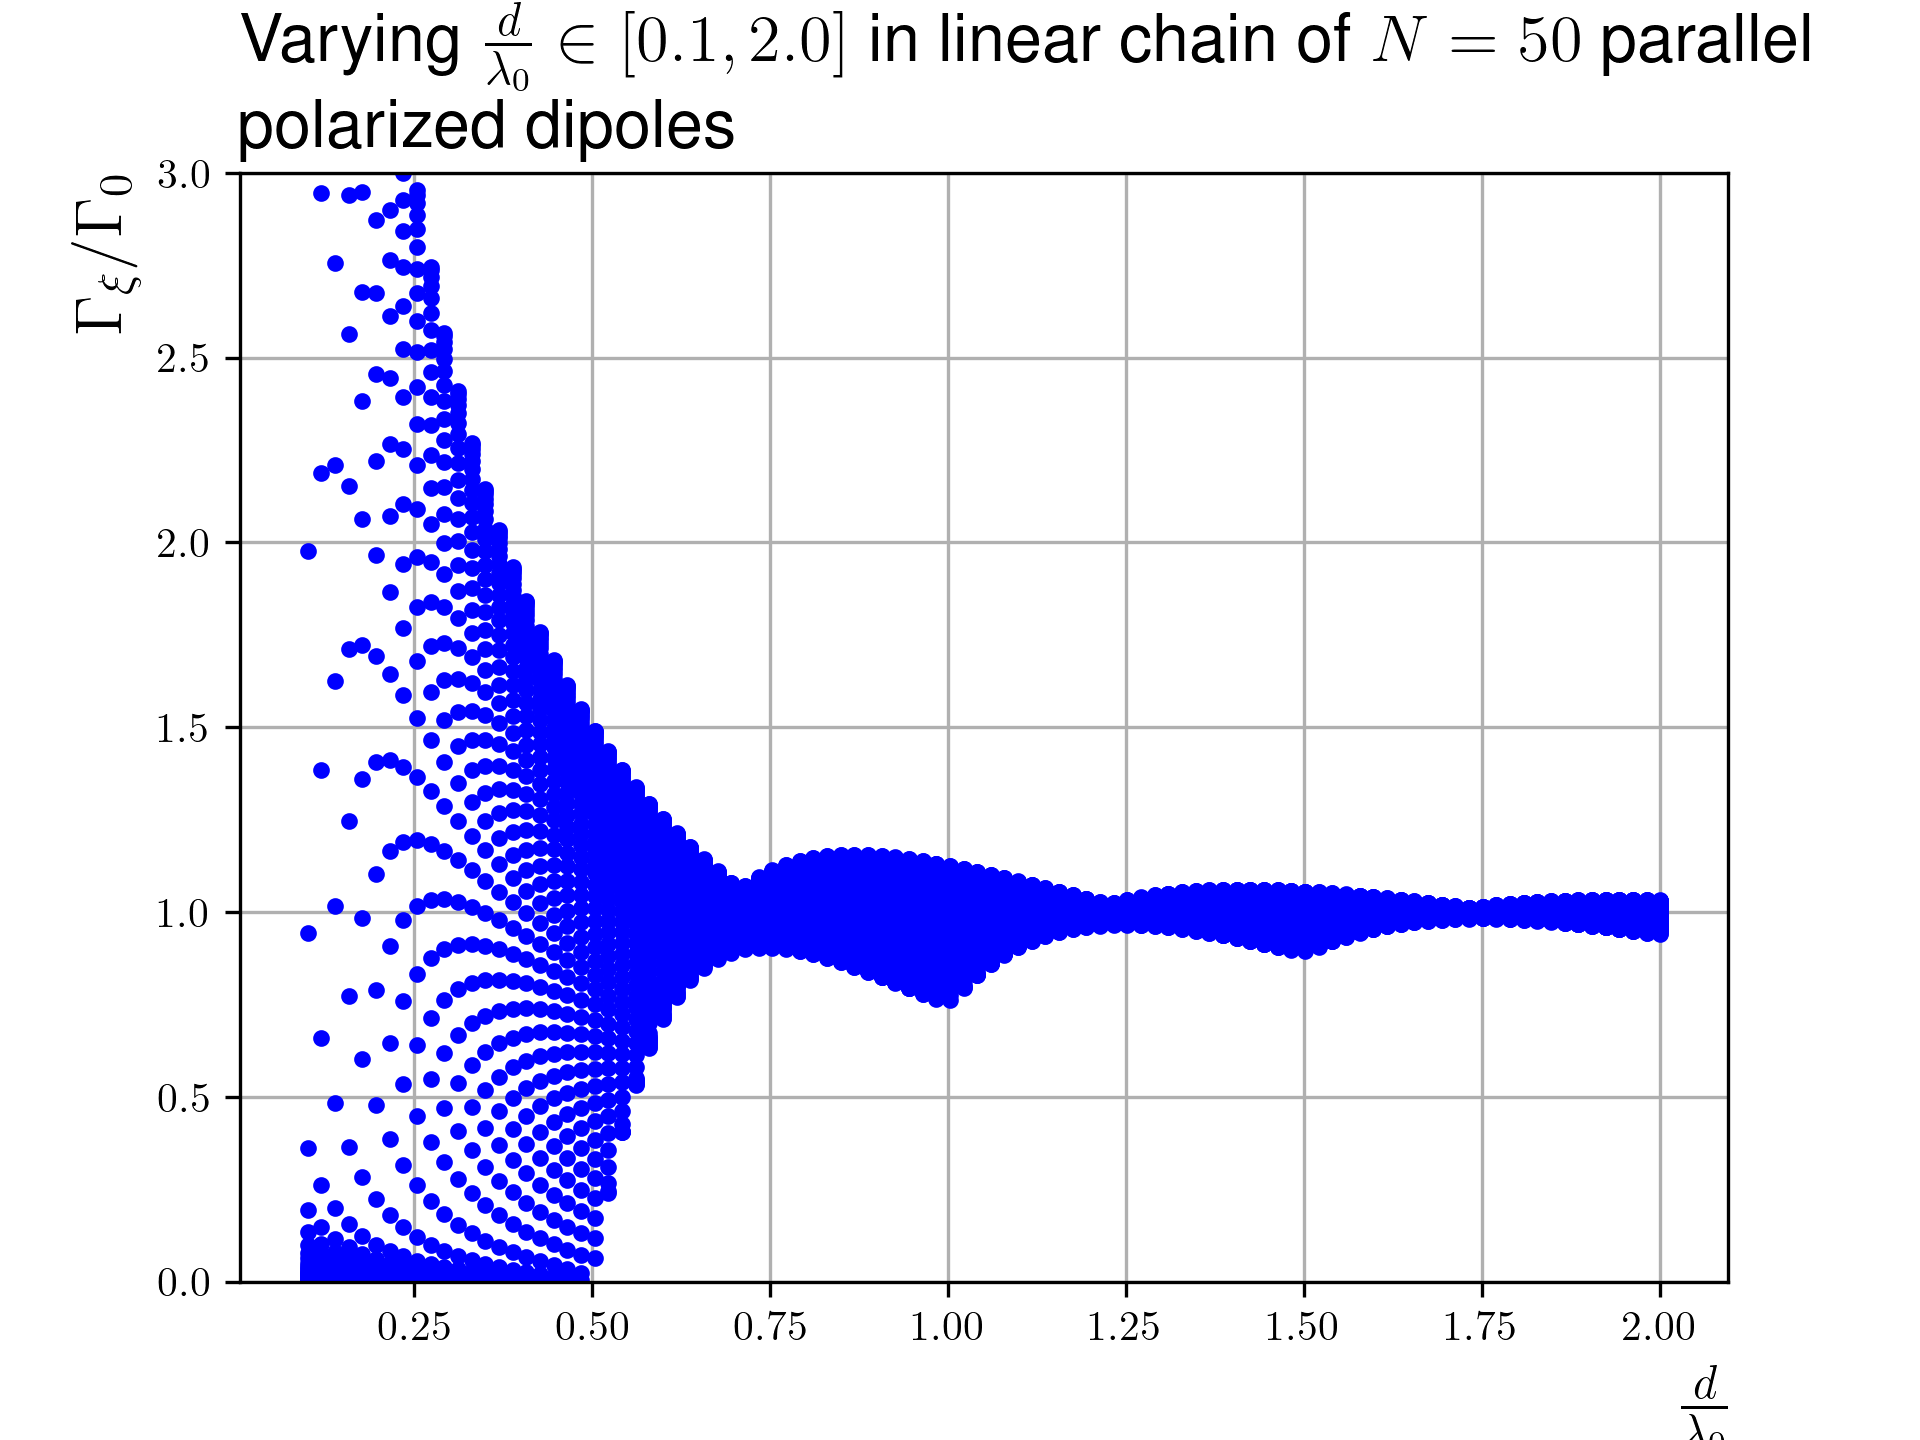
\includegraphics[width=0.75\linewidth]{figs/case_linear_parallel_var_distance_01_2.png}
    \caption{Decay rates of $N=50$ linear chain with dipole moments aligned in parallel to the chain. Each vertical line of points represent the decay rates of the 50 eigenstates at the given distance. Similar tendencies as Figure 3a of (REF Asenjo).}
    \label{fig:linear_chain_decayrates_distance_N50}
\end{figure}

The dipole moments are aligned in parallel to the chain axis. Based on this plot and the production of the other plots of Figure 3 of (REF Asenjo), the computation is verified. In Figure \ref{fig:linear_chain_decayrates_distance_N50}, it is seen that there is no significantly subradiant modes before $\frac{d}{\lambda_0} < 0.5$, i.e. when the distance between the atoms are less than half the wave-length. This property of the system is analytically motivated, as noted in Section IIIA of (REF Asenjo), since the lattice vector must be $d < \frac{\lambda_0}{2}$ to support guided modes in the infinite linear chain. This will serve as a guideline for choosing latticeconstants in the following cases. 

Since the modes of wavevector within the first Brillouin zone are guided modes (REF Asenjo), the only permitted place for the system to emit photons is at the ends of the chain. Therefore, it is hypothesized that the probability amplitude is primarily decreased, when the waves reach the end of the chain. 

God forklaring af figur, der viser a, b, c og d. a: decay rate rangeret, b: most subradiant mode probability amplitude, c: decay rate as function of d og endelig d: as function of N. Xi indexes the modes by decay rates from smallest to greatest. 

\subsubsection{Varying polarization in linear chain}\label{disc:linear_chain_varypola}

Vi ser også i Asenjo IIIA figur 1, at der forventes en mærkeligere opførsel for nogle tilstande, når polarisering er transversal. Måske noget der kan forklare opførslen af de superradiante tilstande. TEORI???

\subsubsection{Broken chain}\label{disc:linear_broken}

\subsection{Circular chain}\label{disc:circular}

The circular lattice is particularly interesting, because the spin-wave modes of the chain never encounters a boundary, which in Section \ref{disc:linear_chain} is the hypothesized primary loss of excited probability amplitude. As seen in (REF Asenjo), the circular lattice's most subradiant mode achieves exponential decrease in decay rate as function of N, $\Gamma_{\xi = 1} \propto e^{-N}$, compared to the linear chain's $\Gamma_{\xi=1} \propto N^{-3}$. But, how does the decay rate change as function of varying the polarization of the chain? First, the circular lattice with most subradiant mode probability amplitude, decay rate as function of interatomic distance and as function of N. 

\subsection{Negative decay rates}

For very small distances, e.g. $\frac{d}{\lambda0} = 0.00001$, the decay rates predicted by the diagonalization of the Hamiltonian can become negative, $a_\xi(t)=e^{-Gamma_\xi t} a_\xi (0) \rightarrow e^{Gamma_\xi t} a_\xi (0)$. This is of course unphysical. As seen, it would mean increase in probability. If the system initialized in a state with negative decay rate, the probability would become greater than 1. Why does it happen for very small interatomic distances? Remember, no assumption was made about the chosen transition. Choosing a microwave transition with optically trapped atoms would e.g. produce such circumstances. 

Forudsigelser for N=2 tilfælde? Problemer! Sammenligning med Adrian N=3 kæde. Vidde på egenværdier gør det svært for algoritmen at være præcis, derfor skal der ikke så meget til, før vi havner på den forkerte side. TEORI?

\subsection{Adressing subradiant states}

TODO: Evt. put noget om, at det er svært at addressere disse subradiante tilstande, og at der indtil videre ikke findes nogle gode protokoller for netop dette (kilde? Udover introduktion in Asenjo-Garcia et al.). 

\subsection{Further research}\label{sec:further}

Other geometries of interest? Helix, . How is decay affected by curvature?
Any specific geometries that make efficient and high-fidelity communication protocols available?

Multiexcitation states and their behaviour (REF, Asenjo-Garcia, Israeli guy)

The framework developed by Grüner \& Welsch (REF) can be extended to include propagation in other media and guided modes. This opens up for other interesting directions to go. E.g. how circular lattices around a fibre with a guided mode acts. How does it affect the decay rates of the system? 

\section{Conclusion}

\newpage
TODO: bibliography

\end{document}